\documentclass[a4paper,12pt]{report}

\usepackage[italian]{babel}
\usepackage{hyperref}
\usepackage[utf8]{inputenc}
\usepackage{float}
\usepackage[table,xcdraw]{xcolor}
\usepackage{longtable}
\usepackage{graphicx}
\usepackage{todonotes}
\usepackage{fancyvrb}

\title{\textbf{Progettazione Database}}
\date{\today}

\begin{document}
	\maketitle
	\tableofcontents
	\chapter{Analisi dei requisiti}
	\section{Introduzione}
	Il progetto ha come obiettivo la realizzazione di una \textbf{piattaforma e-commerce} per la gestione e la vendita di \textbf{scarpe}, con funzionalità di \textbf{tracciamento delle spedizioni}, \textbf{gestione di notifiche per gli utenti} e \textbf{strumenti avanzati di gestione ordini} per gli amministratori. L'intervista seguente esplora i \textbf{requisiti funzionali} e \textbf{non funzionali} del sistema.
	
	\section{Intervista}
	Il progetto prevede la realizzazione di una \textbf{piattaforma e-commerce} che offra \textbf{funzionalità avanzate} sia per gli \textbf{utenti finali} sia per gli \textbf{amministratori del sistema}. Al centro del progetto vi è l’obiettivo di garantire agli utenti una \textbf{navigazione semplice e intuitiva}, permettendo loro di esplorare il \textbf{catalogo prodotti} in modo dettagliato. Si desidera sapere quali \textbf{informazioni devono essere raccolte durante la registrazione degli utenti}, considerando dati essenziali come \textbf{nome}, \textbf{cognome}, \textbf{email} e \textbf{preferenze per ricevere newsletter}. È necessario prevedere un \textbf{sistema che consenta di modificare i dati personali}.
	
	Un altro aspetto fondamentale riguarda il \textbf{catalogo prodotti}, che deve includere \textbf{informazioni complete} su ogni articolo, come il \textbf{nome}, la \textbf{descrizione}, il \textbf{prezzo}, la \textbf{disponibilità} e le \textbf{varianti} relative a \textbf{taglia} e \textbf{colore}. L’utente deve poter \textbf{filtrare} e \textbf{cercare i prodotti} in base a criteri come il \textbf{brand}, il \textbf{tipo} e la \textbf{fascia di prezzo}. La \textbf{gestione del carrello} è un elemento centrale: i prodotti nel carrello vengono mantenuti nel tempo solo per gli \textbf{utenti registrati} e come debbano essere gestiti eventuali \textbf{sconti} o \textbf{promozioni} applicabili al momento del pagamento. Inoltre, l’interfaccia deve permettere di \textbf{aggiungere}, \textbf{modificare} o \textbf{rimuovere articoli} in modo rapido e intuitivo.
	
	Per quanto riguarda gli \textbf{ordini}, si richiede che il sistema consenta agli utenti di \textbf{visualizzare uno storico dettagliato}, includendo informazioni sui \textbf{prodotti acquistati}, il \textbf{costo totale} e lo \textbf{stato della spedizione}. È necessario definire quali \textbf{stati debbano essere inclusi nel tracciamento delle spedizioni} e come questi cambiamenti debbano essere \textbf{notificati agli utenti}. Si richiede che le \textbf{notifiche} siano inviate non solo tramite il \textbf{portale}, ma anche via \textbf{email}, per garantire una comunicazione tempestiva, specialmente per \textbf{eventi critici} come \textbf{conferme d’ordine} o \textbf{aggiornamenti sul tracking della spedizione}.
	
	La piattaforma deve inoltre prevedere \textbf{funzionalità di gestione per la wishlist}, dove gli utenti possono \textbf{salvare prodotti di interesse} e \textbf{ricevere notifiche} su eventuali \textbf{cambi di prezzo} o \textbf{disponibilità}. Un’altra funzionalità richiesta è la \textbf{possibilità di recensire i prodotti acquistati}, con un \textbf{sistema che consenta di assegnare un punteggio e aggiungere commenti}, contribuendo a una \textbf{sezione di feedback} visibile ad altri utenti.
	
	Dal lato \textbf{amministrativo}, è necessario definire un \textbf{pannello di controllo} che permetta la \textbf{gestione completa del catalogo}, con la possibilità di \textbf{aggiungere}, \textbf{rimuovere} o \textbf{modificare prodotti}, comprese le \textbf{varianti}. Si richiede che ogni \textbf{modifica}, in particolare quelle sui \textbf{prezzi}, sia \textbf{tracciata} per garantire uno \textbf{storico dettagliato}. Per la \textbf{gestione degli ordini}, gli amministratori devono poter \textbf{visualizzare}, \textbf{aggiornare lo stato delle spedizioni} e \textbf{segnare gli ordini come completati}. Un altro aspetto rilevante è la \textbf{gestione dei codici sconto}: gli amministratori devono poter \textbf{attivare}, \textbf{modificare} e \textbf{disattivare sconti}, specificando \textbf{parametri} come la \textbf{percentuale applicabile}, la \textbf{validità} e il \textbf{limite massimo di utilizzi}.
	
	Infine, dal punto di vista \textbf{comunicativo}, il sistema deve consentire agli utenti di \textbf{inviare messaggi agli amministratori} tramite un \textbf{form dedicato}. Gli amministratori devono poter \textbf{visualizzare questi messaggi} e \textbf{rispondere tramite email}. È richiesto anche un \textbf{sistema di generazione di report} che consenta agli amministratori di \textbf{visualizzare statistiche} sui \textbf{ricavi}, i \textbf{prodotti più venduti} e l’\textbf{andamento generale delle vendite}.
	
	Un aspetto critico è la \textbf{sicurezza del sistema}, che deve garantire la \textbf{protezione dei dati degli utenti}, con misure come la \textbf{crittografia delle password}. È importante considerare anche la \textbf{scalabilità della piattaforma}, per gestire eventuali \textbf{aumenti nel numero di utenti e prodotti} in futuro.
	
	\section{Rielaborazione del Testo}
	\subsection{Obiettivi finali:}
	Il sistema deve consentire agli \textbf{utenti} di accedere alla piattaforma per \textbf{esplorare} e \textbf{acquistare scarpe}, offrendo un'esperienza \textbf{semplice e intuitiva}. Devono essere implementate \textbf{funzionalità per la gestione del catalogo prodotti}, con possibilità di \textbf{filtrare} e \textbf{cercare articoli} in base a vari criteri come \textbf{marca}, \textbf{prezzo}, \textbf{taglia} e \textbf{colore}. \\
	Per incentivare gli utenti a interagire con la piattaforma, è prevista una \textbf{funzionalità di recensione dei prodotti}, dove gli utenti possono \textbf{valutare gli articoli acquistati} e \textbf{lasciare commenti}. Tali recensioni possono contribuire a una \textbf{sezione dedicata al feedback complessivo} sui prodotti. \\
	Dal lato amministrativo, il sistema deve permettere la \textbf{gestione centralizzata del catalogo}, degli \textbf{ordini} e delle \textbf{promozioni}. Gli amministratori devono avere accesso a \textbf{strumenti per monitorare le vendite}, \textbf{aggiornare le informazioni sui prodotti} e \textbf{gestire i codici sconto}. Devono essere disponibili anche \textbf{statistiche} per visualizzare i \textbf{ricavi} e i \textbf{prodotti più venduti}.
	
	\section{Estrazione dei dati del testo rielaborato}
	\subsection{Estrazione dati sugli utenti}
	\textbf{Utente} $\longrightarrow$ Utente che si registra sulla piattaforma\\
	Successivamente verranno elencati i dati da memorizzare.
	\begin{itemize}
		\item Password
		\item Nome
		\item Cognome
		\item Email
		\item Preferenze per la newsletter
	\end{itemize}
	
	\textbf{Amministratore} $\longrightarrow$ Utente privilegiato che effettua operazioni di moderazione e gestione dei dati.\\
	Successivamente verranno elencati i dati da memorizzare.
	\begin{itemize}
		\item Password
		\item Nome
		\item Cognome
		\item Email
		\item Telefono
	\end{itemize}
	
	\textbf{Prodotti} $\longrightarrow$ Scarpe disponibili per la vendita.\\
	Successivamente verranno elencati i dati da memorizzare.
	\begin{itemize}
		\item Nome
		\item Descrizione
		\item Prezzo
		\item Taglia
		\item Colore
		\item Brand
		\item Disponibilità
	\end{itemize}
	
	\section{Elenco delle Azioni}
	\subsection{Utente}
	\begin{itemize}
		\item \textbf{Registrarsi sulla piattaforma}.
		\item \textbf{Accedere alla piattaforma}.
		\item \textbf{Navigare e filtrare i prodotti} (per brand, tipo di calzatura, taglia, colore, prezzo, etc.).
		\item \textbf{Aggiungere/consultare/modificare i prodotti in un carrello}.
		\item \textbf{Pagare i prodotti nel carrello}.
		\item \textbf{Consultare/modificare le notifiche} (segna come letto, elimina).
		\item \textbf{Modificare i propri dati tramite un pannello delle impostazioni}.
		\item \textbf{Consultare lo stato della spedizione}.
		\item \textbf{Visualizzare lo storico degli ordini}.
		\item \textbf{Visualizzare il grafico dell’andamento del prezzo di ogni articolo} (e prezzo più basso).
		\item \textbf{Tracking della Spedizione}.
		\item \textbf{Gestire la lista dei desideri}.
		\item \textbf{Ricevere le notifiche anche nella mail}.
		\item \textbf{Recensire i prodotti} (stelle e media + sezione con commenti).
		\item \textbf{Contattare l’admin tramite un form}.
		\item \textbf{Gestire l’iscrizione alla newsletter nel pannello}.
		\item \textbf{Iscriversi alla newsletter} per ricevere email su sconti, novità etc.
		\item \textbf{Ricevere notifiche tramite mail} al cambio dello stato di spedizione, su carrelli abbandonati, cambio prezzo di articoli in wishlist e per conferme d’ordine.
	\end{itemize}
	\subsection{Amministratore}
	\begin{itemize}
		\item \textbf{Utilizzare un pannello per la gestione dei prodotti} (aggiungere/rimuovere prodotti, modificare i prezzi).
		\item \textbf{Gestione degli ordini}.
		\begin{itemize}
			\item \textbf{Ordini appena ricevuti} (segnare come spediti).
			\item \textbf{Ordini spediti} (in automatico nello storico quando ricevuti).
			\item \textbf{Storico ordini}.
		\end{itemize}
		\item \textbf{Aggiornare le informazioni del venditore visualizzate sul sito} (e.g., indirizzo, numero di telefono nel footer).
		\item \textbf{Generare statistiche sui ricavi}.
		\item \textbf{Attivare codici sconto} (da inserire nel Database).
		\item \textbf{Gestire i messaggi ricevuti dagli utenti} (la cui risposta dovrà essere mandata alla mail del mittente).
	\end{itemize}
	
	\chapter{Progettazione concettuale}
	\subsection{Schema completo}
	\begin{figure}[H]
		\centering
		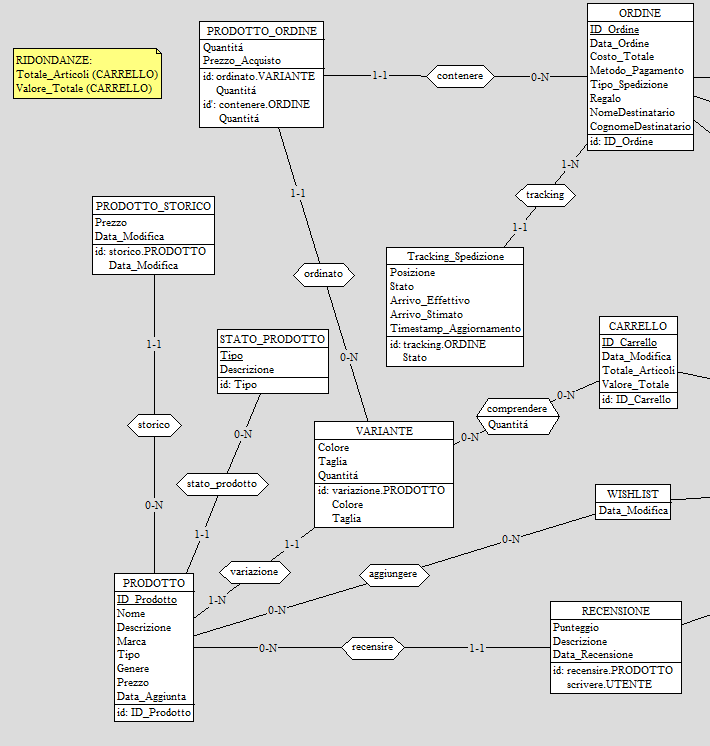
\includegraphics[width=400pt]{ER/er_completo_sx.png}
		\caption{Schema ER completo 1/2.}
	\end{figure}
	\begin{figure}[H]
		\centering
		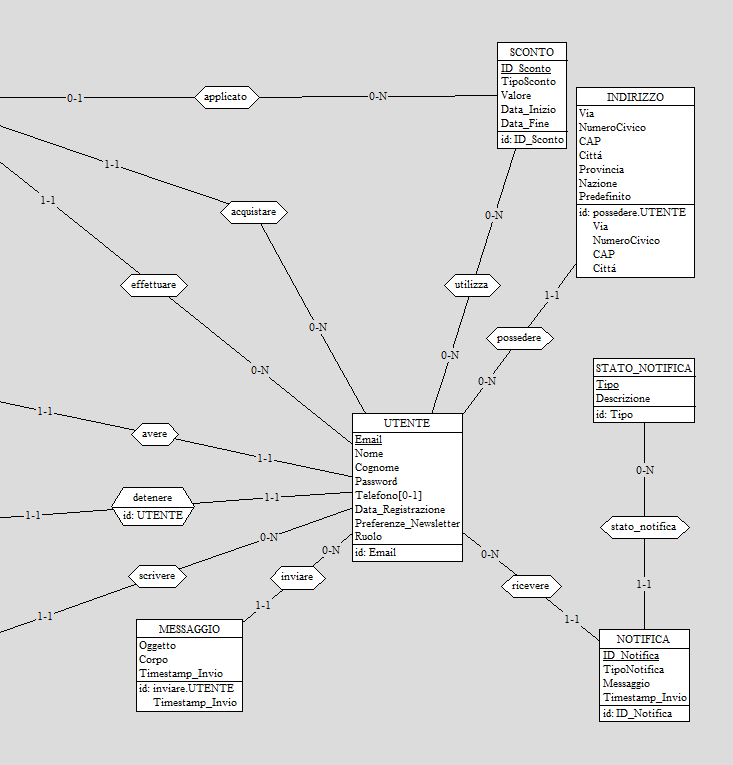
\includegraphics[width=400pt]{ER/er_completo_dx.png}
		\caption{Schema ER completo 2/2.}
	\end{figure}
	
	\chapter{Progettazione Logica}
	\section{Stima del volume dei dati} \label{s:volumes}
	\begin{table}[H]
		\centering
		\begin{tabular}{|lll|}
			\hline
			\rowcolor[HTML]{FFCE93}
			\multicolumn{3}{|l|}{\cellcolor[HTML]{FFCE93}Utenti e Notifiche} \\ \hline
			\rowcolor[HTML]{CBCEFB}
			Concetto            & Costrutto & Volume           \\ \hline
			UTENTE              & E         & 100000           \\ \hline
			MESSAGGIO           & E         & 10000            \\ \hline
			NOTIFICA            & E         & 50000            \\ \hline
			STATO\_NOTIFICA     & E         & 3                \\ \hline
			PAGAMENTO			& E 		& 50000			   \\ \hline
			INDIRIZZO			& E			& 100000		   \\ \hline
			stato\_notifica     & R         & 50000            \\ \hline
			intestato			& R			& 50000			   \\ \hline
			possedere			& R   		& 100000		   \\ \hline
			inviare             & R         & 10000            \\ \hline
			ricevere            & R         & 50000            \\ \hline
			effettuare          & R         & 200000           \\ \hline
			avere          		& R         & 10000            \\ \hline
			detenere            & R         & 5000             \\ \hline
		\end{tabular}
		\caption{Volume dei dati per utenti e notifiche.}
	\end{table}
	
	\begin{table}[H]
		\centering
		\begin{tabular}{|lll|}
			\hline
			\rowcolor[HTML]{FFCE93}
			\multicolumn{3}{|l|}{\cellcolor[HTML]{FFCE93}Prodotti e Varianti} \\ \hline
			\rowcolor[HTML]{CBCEFB}
			Concetto          & Costrutto & Volume           \\ \hline
			PRODOTTO          & E         & 10000            \\ \hline
			VARIANTE          & E         & 30000            \\ \hline
			STATO\_PRODOTTO   & E         & 5                \\ \hline
			PRODOTTO\_STORICO & E         & 30000            \\ \hline
			stato\_prodotto   & R         & 10000            \\ \hline
			variazione        & R         & 30000            \\ \hline
			storico           & R         & 30000            \\ \hline
		\end{tabular}
		\caption{Volume dei dati per prodotti e varianti.}
	\end{table}
	
	\begin{table}[H]
		\centering
		\begin{tabular}{|lll|}
			\hline
			\rowcolor[HTML]{FFCE93}
			\multicolumn{3}{|l|}{\cellcolor[HTML]{FFCE93}Ordini e Carrelli} \\ \hline
			\rowcolor[HTML]{CBCEFB}
			Concetto          		& Costrutto & Volume           \\ \hline
			ORDINE            		& E         & 200000           \\ \hline
			TRACKING\_SPEDIZIONE 	& E      	& 200000           \\ \hline
			STATO\_SPEDIZIONE   	& E         & 5                \\ \hline
			PRODOTTO\_ORDINE  		& R         & 600000           \\ \hline
			CARRELLO          		& E         & 20000            \\ \hline
			stato\_spedizione   	& R         & 200000           \\ \hline
			ordinato				& R			& 600000 		   \\ \hline
			comprendere       		& R         & 20000            \\ \hline
			tracking 				& R      	& 200000           \\ \hline
			contenere 				& R      	& 600000           \\ \hline
		\end{tabular}
		\caption{Volume dei dati per ordini e carrelli.}
	\end{table}
	
	\begin{table}[H]
		\centering
		\begin{tabular}{|lll|}
			\hline
			\rowcolor[HTML]{FFCE93}
			\multicolumn{3}{|l|}{\cellcolor[HTML]{FFCE93}Wishlist e Recensioni} \\ \hline
			\rowcolor[HTML]{CBCEFB}
			Concetto          & Costrutto & Volume           \\ \hline
			WISHLIST          & E         & 150000           \\ \hline
			RECENSIONE        & E         & 200000           \\ \hline
			aggiungere        & R         & 150000           \\ \hline
			scrivere          & R         & 200000           \\ \hline
			recensire         & R         & 200000           \\ \hline
		\end{tabular}
		\caption{Volume dei dati per wishlist e recensioni.}
	\end{table}
	
	\begin{table}[H]
		\centering
		\begin{tabular}{|lll|}
			\hline
			\rowcolor[HTML]{FFCE93}
			\multicolumn{3}{|l|}{\cellcolor[HTML]{FFCE93}Sconti e Promozioni} \\ \hline
			\rowcolor[HTML]{CBCEFB}
			Concetto          & Costrutto & Volume           \\ \hline
			SCONTO            & E         & 1000             \\ \hline
			applicato         & R         & 20000            \\ \hline
			utilizza          & R         & 10000            \\ \hline
		\end{tabular}
		\caption{Volume dei dati per sconti e promozioni.}
	\end{table}
	\section{Operazioni e loro frequenza}
	\subsection{Operazioni dell'utenza}
	\begin{small}
		\begin{longtable}[H]{|c|p{5cm}|>{\columncolor[HTML]{FFFFC7}}p{2.5cm}|p{5cm}|}
			\hline
			\cellcolor[HTML]{ECF4FF}Numero & 
			\cellcolor[HTML]{ECF4FF}Operazione & 
			\cellcolor[HTML]{ECF4FF}Frequenza / gg & 
			\cellcolor[HTML]{ECF4FF}Dettagli \\ \hline
			\endfirsthead
			\endhead
			%
			1 & Registrazione di un nuovo utente. & 10 & Numero medio di nuovi utenti al giorno. \\ \hline
			2 & Accesso alla piattaforma. & 100 & Stimato considerando il numero medio di utenti attivi. \\ \hline
			3 & Navigazione e filtraggio dei prodotti. & 200 & Include filtri per brand, tipo, taglia, colore, prezzo, ecc. \\ \hline
			4 & Aggiunta, consultazione o modifica di prodotti nel carrello. & 150 & Utenti che interagiscono con il carrello ogni giorno. \\ \hline
			5 & Pagamento dei prodotti nel carrello. & 50 & Basato sulla conversione media degli utenti. \\ \hline
			6 & Consultazione o modifica delle notifiche. & 80 & Utenti che interagiscono con le notifiche. \\ \hline
			7 & Modifica dei propri dati nel pannello impostazioni. & 20 & Include aggiornamento di password, telefono, ecc. \\ \hline
			8 & Consultazione dello stato della spedizione. & 70 & Stimato sulla base degli ordini recenti. \\ \hline
			9 & Visualizzazione dello storico degli ordini. & 50 & Utenti che consultano i propri ordini passati. \\ \hline
			10 & Visualizzazione del grafico dell’andamento del prezzo. & 40 & Per articoli specifici in wishlist o nel carrello. \\ \hline
			11 & Tracking della spedizione. & 50 & Utenti che controllano lo stato aggiornato del tracking. \\ \hline
			12 & Gestione della lista dei desideri. & 30 & Aggiunta o rimozione di articoli dalla wishlist. \\ \hline
			13 & Ricezione delle notifiche tramite email. & 100 & Include notifiche su ordini, spedizioni, e wishlist. \\ \hline
			14 & Recensioni dei prodotti (stelle e commenti). & 20 & Basato sugli utenti che lasciano recensioni giornalmente. \\ \hline
			15 & Contattare l’amministratore tramite un form. & 5 & Utenti che inviano richieste o segnalazioni. \\ \hline
			16 & Gestione dell’iscrizione alla newsletter. & 10 & Include iscrizioni e cancellazioni. \\ \hline
			17 & Iscrizione alla newsletter. & 10 & Numero medio di nuove iscrizioni giornaliere. \\ \hline
		\end{longtable}
	\end{small}
	
	\subsection{Operazioni di amministrazione}
	\begin{small}
		\begin{longtable}[H]{|c|p{5cm}|>{\columncolor[HTML]{FFFFC7}}p{2.5cm}|p{5cm}|}
			\hline
			\cellcolor[HTML]{ECF4FF}Numero & 
			\cellcolor[HTML]{ECF4FF}Operazione & 
			\cellcolor[HTML]{ECF4FF}Frequenza & 
			\cellcolor[HTML]{ECF4FF}Dettagli \\ \hline
			\endfirsthead
			\endhead
			%
			1 & Gestione dei prodotti (aggiunta/rimozione/modifica). & 5 / settimana & Operazioni su nuovi prodotti o modifica dei prezzi esistenti. \\ \hline
			2 & Gestione degli ordini. & 50 / giorno & Include ordini appena ricevuti, spediti e storicizzati. \\ \hline
			3 & Aggiornamento delle informazioni del venditore. & 2 / mese & Modifica di indirizzi o informazioni di contatto nel footer. \\ \hline
			4 & Generazione di statistiche sui ricavi. & 1 / settimana & Report su ricavi e vendite complessive. \\ \hline
			5 & Attivazione di codici sconto. & 3 / mese & Inserimento di nuove promozioni nel database. \\ \hline
			6 & Gestione dei messaggi ricevuti dagli utenti. & 10 / giorno & Risposte inviate via mail agli utenti. \\ \hline
		\end{longtable}
	\end{small}
	
	\section{Analisi delle ridondanze}
	Le ridondanze principali che vogliamo analizzare sono le seguenti:
	\begin{enumerate}
		\item Attributo "Totale\_Articoli" nell'entità CARRELLO.
		\item Attributo "Valore\_Totale" nell'entità CARRELLO.
	\end{enumerate}
	
	\subsection{Attributo 1: Totale\_Articoli}
	\subsubsection{Operazioni interessate:}
	\begin{itemize}
		\item Op. 4: Aggiunta, consultazione o modifica di prodotti nel carrello.
		\item Op. 5: Pagamento dei prodotti nel carrello.
	\end{itemize}
	
	\subsubsection{Tabelle degli accessi senza ridondanza:}
	Consideriamo il caso in cui il calcolo di "Totale\_Articoli" venga effettuato dinamicamente ogni volta che è necessario.
	
	\begin{itemize}
		\item \textbf{Per operazione 4}: Per ogni modifica al carrello (aggiunta o rimozione di un prodotto), sono necessarie $150$ scritture nella relazione "comprendere" e $150$ letture per ricalcolare "Totale\_Articoli". Scritture: $150 \times 2 = 300$ accessi. Letture: $150 \times 1 = 150$ accessi. Totale: $300 + 150 = 450$ accessi/giorno.
		\item \textbf{Per operazione 5}: Per il pagamento, vengono effettuate $50$ letture per calcolare dinamicamente "Totale\_Articoli". Letture: $50 \times 1 = 50$ accessi. Totale: $450 + 50 = 500$ accessi/giorno.
	\end{itemize}
	
	\subsubsection{Tabelle degli accessi con ridondanza:}
	Consideriamo il caso in cui si introduca un attributo ridondante "Totale\_Articoli" nell'entità CARRELLO, che viene aggiornato ogni volta che il contenuto del carrello viene modificato.
	
	\begin{itemize}
		\item \textbf{Per operazione 4}: Oltre alle $150$ scritture nella relazione "comprendere", sono necessari $150$ aggiornamenti sull'entità CARRELLO. Scritture: $(150 + 150) \times 2 = 600$ accessi. Totale: $600$ accessi/giorno.
		\item \textbf{Per operazione 5}: Per il pagamento, vengono effettuate $50$ letture dirette di "Totale\_Articoli", senza necessità di ricalcolo. Letture: $50 \times 1 = 50$ accessi. Totale: $600 + 50 = 650$ accessi/giorno.
	\end{itemize}
	
	\subsubsection{Conclusione:}
	\begin{itemize}
		\item \textbf{Senza ridondanza}: $500$ accessi/giorno.
		\item \textbf{Con ridondanza}: $650$ accessi/giorno.
	\end{itemize}
	Risulta più conveniente \textbf{eliminare la ridondanza}, poiché il costo aggiuntivo delle scritture è significativo rispetto alla riduzione delle letture.
	
	\subsection{Attributo 2: Valore\_Totale}
	\subsubsection{Operazioni interessate:}
	\begin{itemize}
		\item Op. 4: Aggiunta, consultazione o modifica di prodotti nel carrello.
		\item Op. 5: Pagamento dei prodotti nel carrello.
	\end{itemize}
	
	\subsubsection{Tabelle degli accessi senza ridondanza:}
	Consideriamo il caso in cui il calcolo di "Valore\_Totale" venga effettuato dinamicamente ogni volta che è necessario, sommando i prezzi di tutti i prodotti nel carrello.
	
	\begin{itemize}
		\item \textbf{Per operazione 4}: Ogni modifica al carrello richiede $150$ scritture nella relazione "comprendere" e $300$ letture per ricalcolare "Valore\_Totale". Scritture: $150 \times 2 = 300$ accessi. Letture: $300 \times 1 = 300$ accessi. Totale: $300 + 300 = 600$ accessi/giorno.
		\item \textbf{Per operazione 5}: Per il pagamento, vengono effettuate $100$ letture per calcolare dinamicamente "Valore\_Totale". Letture: $100 \times 1 = 100$ accessi. Totale: $600 + 100 = 700$ accessi/giorno.
	\end{itemize}
	
	\subsubsection{Tabelle degli accessi con ridondanza:}
	Consideriamo il caso in cui si introduca un attributo ridondante "Valore\_Totale" nell'entità CARRELLO, che viene aggiornato ogni volta che il contenuto del carrello viene modificato.
	
	\begin{itemize}
		\item \textbf{Per operazione 4}: Ogni modifica al carrello comporta $150$ scritture nella relazione "comprendere" e $150$ aggiornamenti sull'entità CARRELLO. Scritture: $(150 + 150) \times 2 = 600$ accessi. Totale: $600$ accessi/giorno.
		\item \textbf{Per operazione 5}: Per il pagamento, vengono effettuate $50$ letture dirette di "Valore\_Totale", senza necessità di ricalcolo. Letture: $50 \times 1 = 50$ accessi. Totale: $600 + 50 = 650$ accessi/giorno.
	\end{itemize}
	
	\subsubsection{Conclusione:}
	\begin{itemize}
		\item \textbf{Senza ridondanza}: $700$ accessi/giorno.
		\item \textbf{Con ridondanza}: $650$ accessi/giorno.
	\end{itemize}
	Risulta più conveniente \textbf{mantenere la ridondanza}, poiché riduce leggermente il numero totale di accessi.
	
	\section{Conclusioni finali sull'analisi delle ridondanze}
	Dall'analisi delle ridondanze sui tre attributi considerati (\textbf{Totale\_Articoli} e \textbf{Valore\_Totale}, possiamo trarre le seguenti conclusioni:
	\begin{itemize}
		\item \textbf{Totale\_Articoli}: Risulta conveniente \textbf{eliminare la ridondanza}, poiché il costo aggiuntivo delle scritture supera il beneficio della riduzione delle letture.
		\item \textbf{Valore\_Totale}: Risulta conveniente \textbf{mantenere la ridondanza}, poiché riduce il numero totale di accessi.
	\end{itemize}
	\begin{figure}[H]
		\centering
		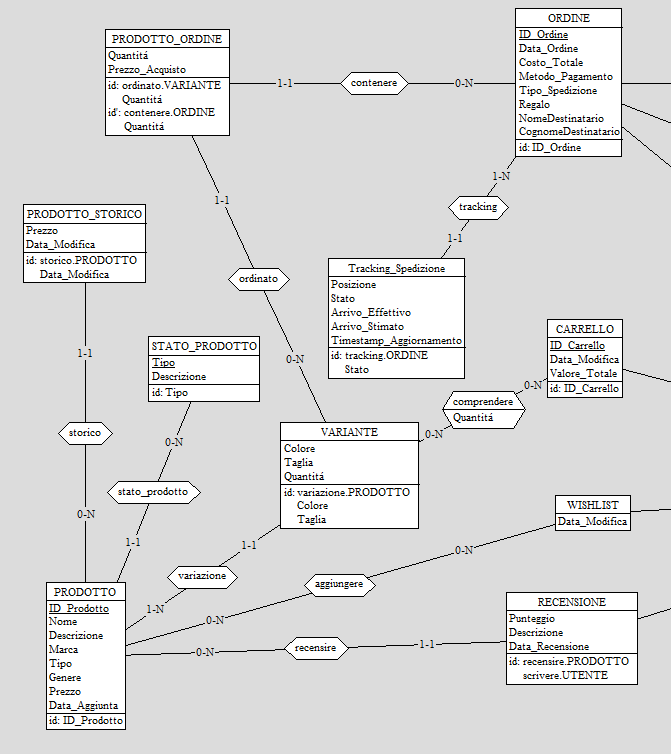
\includegraphics[width=400pt]{ER/er_finale_sx.png}
		\caption{Schema ER finale 1/2.}
	\end{figure}
	\begin{figure}[H]
		\centering
		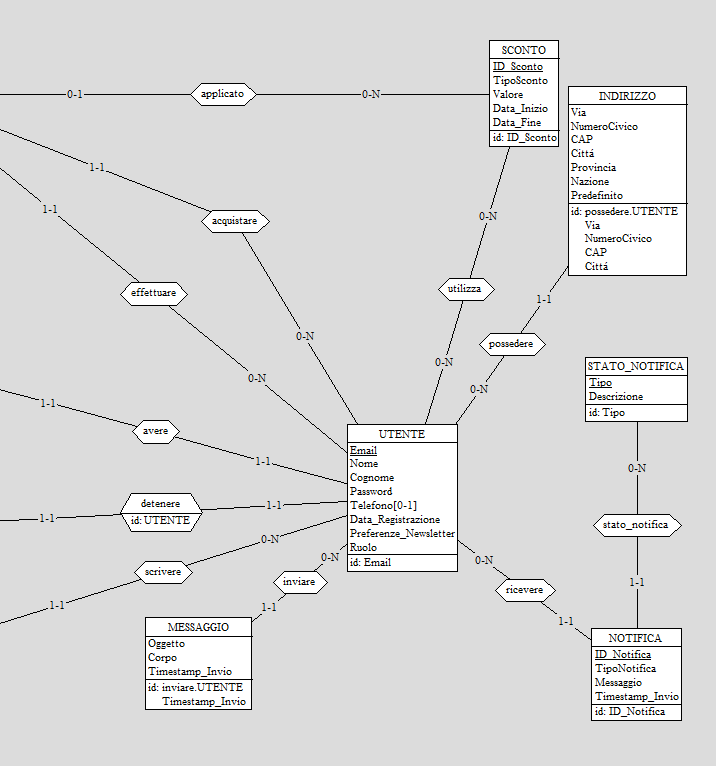
\includegraphics[width=400pt]{ER/er_finale_dx.png}
		\caption{Schema ER finale 2/2.}
	\end{figure}
	
	\section{Traduzione di entità e associazioni in relazioni}
	\subsection{Schema tradotto}
	\begin{figure}[H]
		\centering
		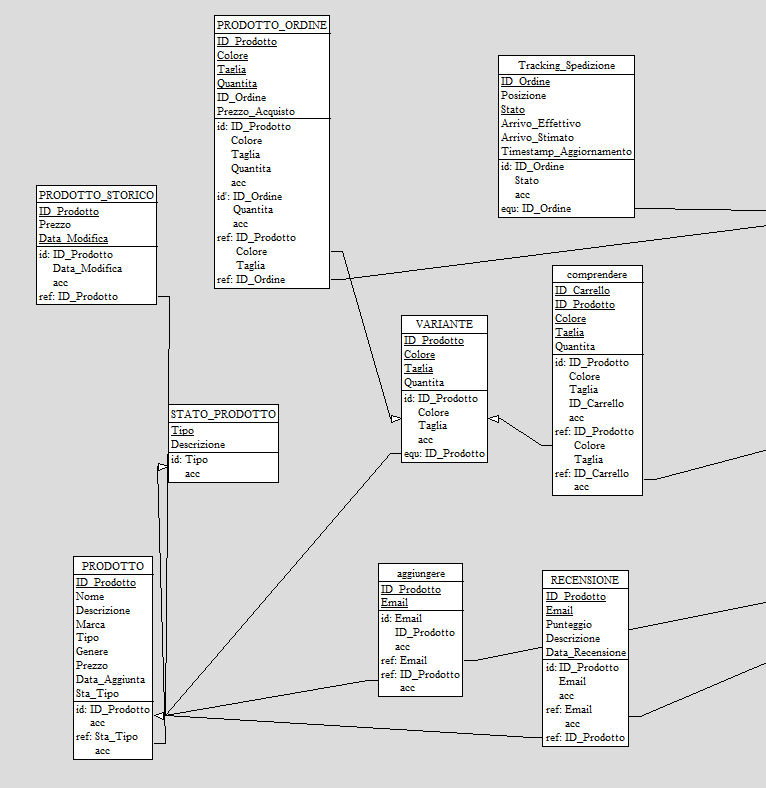
\includegraphics[width=400pt]{ER/Logic/rel_sx.png}
		\caption{Schema Logico 1/2.}
	\end{figure}
	\begin{figure}[H]
		\centering
		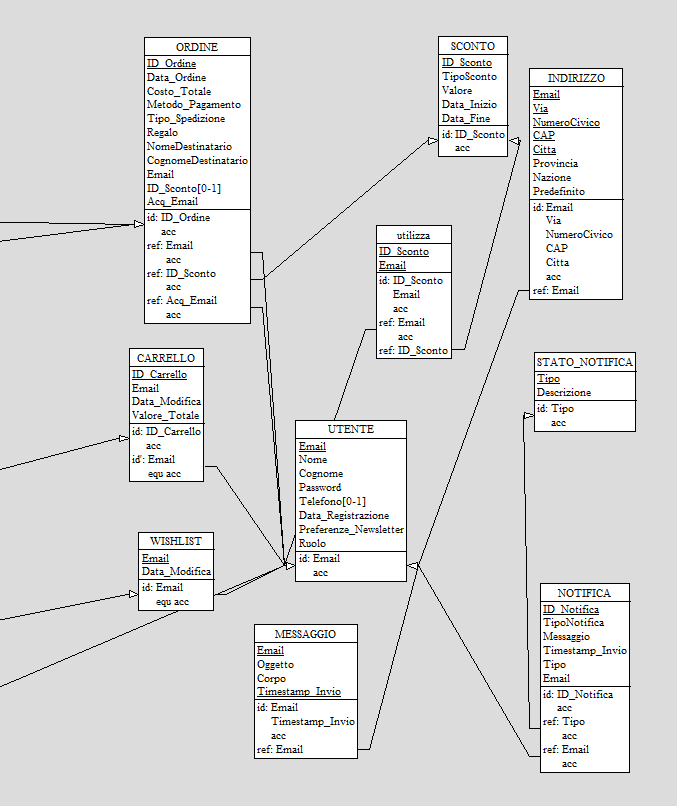
\includegraphics[width=400pt]{ER/Logic/rel_dx.png}
		\caption{Schema Logico 2/2.}
	\end{figure}
\end{document}
